\section{General discussion}

\begin{frame}
\frametitle{Environmental correlations and forecasting \Discussion}

\textbf{Can plants `predict' the arrival of the cold season?\\
 What sources of information do they use?}

    \centering
    \includegraphics[height=0.75\textheight]{../photos/winter}
\end{frame}

\begin{frame}
\frametitle{Environmental correlations and forecasting \Discussion}

\textbf{Can plants `predict' the arrival of the spring?\\
 What sources of information do they use?}

    \centering
    \includegraphics[height=0.75\textheight]{../photos/spring}
\end{frame}

\begin{frame}
\frametitle{Environmental correlations and forecasting \Discussion}

\textbf{Can plants emit `signals' for their benefit?\\
What are the signals used to attract pollinators?}

    \centering
    \includegraphics[height=0.75\textheight]{../photos/bumblebee}
\end{frame}

\begin{frame}
\frametitle{Environmental correlations and forecasting \Discussion}

\textbf{Can plants emit `signals' for their benefit?\\
What are the signals used to enlist ``helpers'' for seed dispersal?}

    \centering
    \includegraphics[height=0.75\textheight]{../photos/berry_eater}
\end{frame}

\begin{frame}
\frametitle{Environmental correlations and forecasting \Discussion}

\textbf{Can plants emit signals to deceive other organisms?\\
How does mimicry work?}

    \centering
    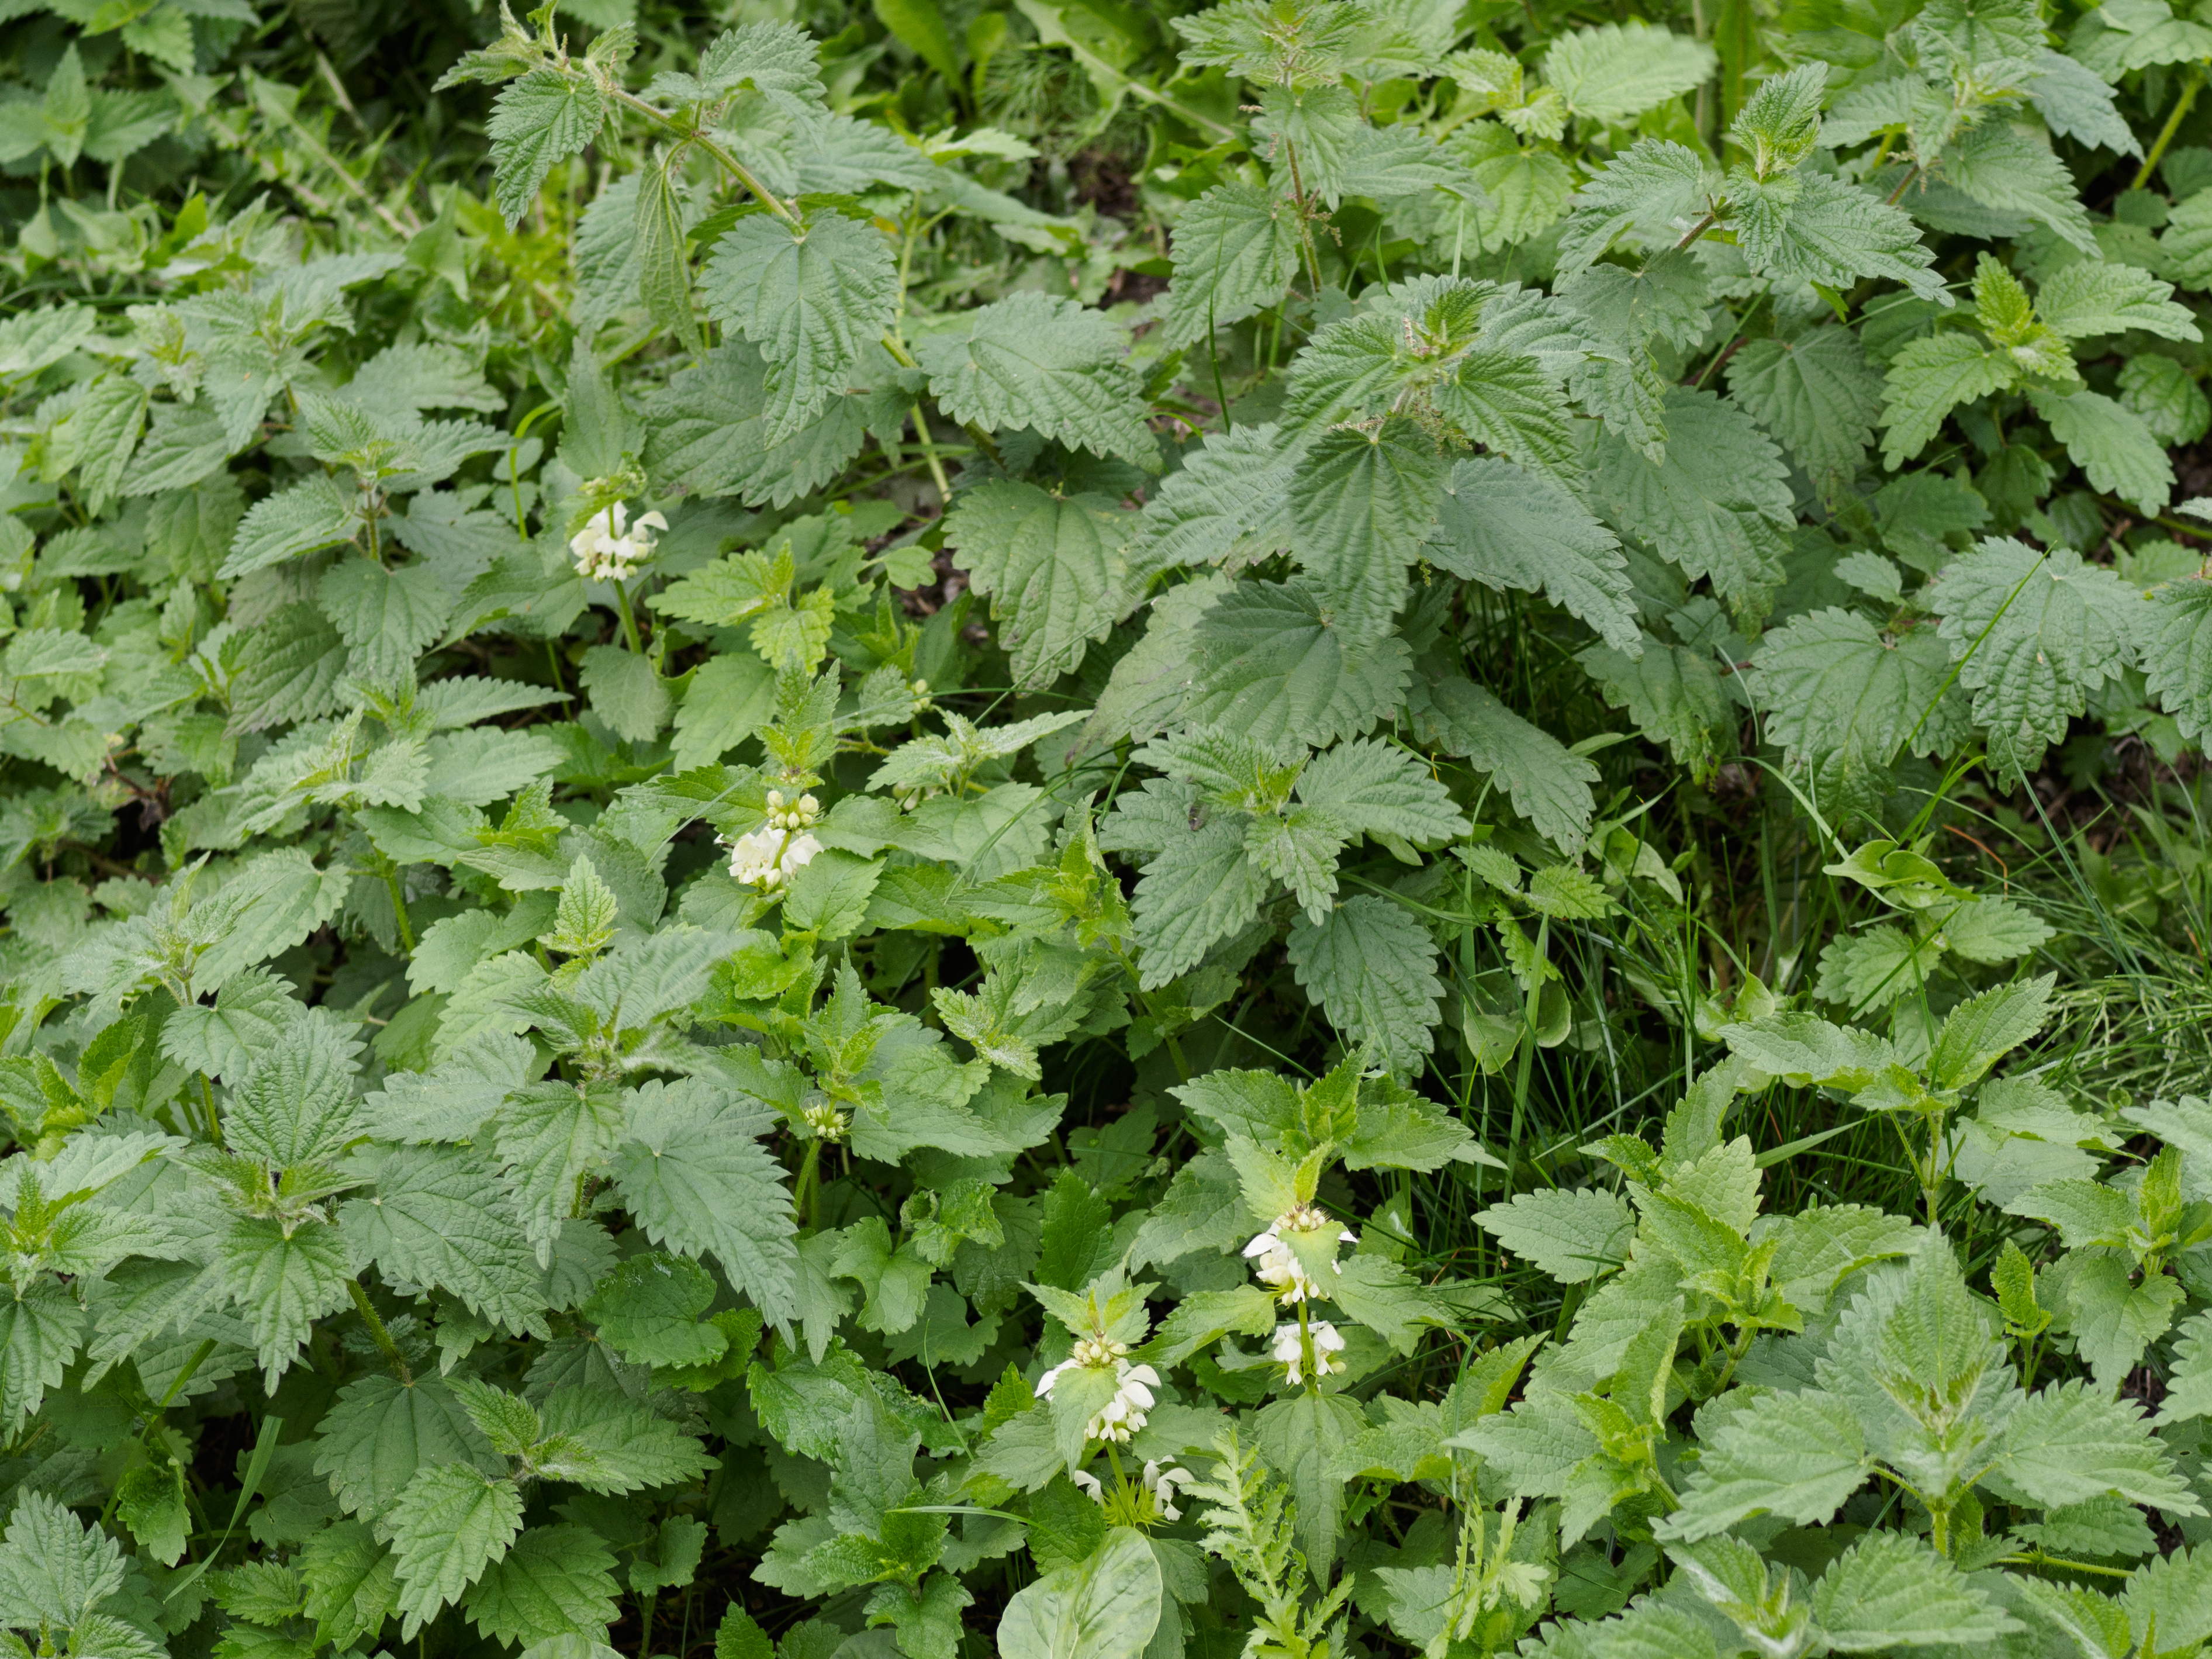
\includegraphics[height=0.75\textheight]{../photos/nettle}
\end{frame}

\begin{frame}
\frametitle{Environmental correlations and forecasting \Discussion}

\textbf{Can plants `generate' environmental correlations for their benefit?\\
How does release of organic volatile compounds create a correlation?}

    \centering
    \includegraphics[height=0.7\textheight]{../photos/aphids}
\end{frame}

\begin{frame}
\frametitle{Symbioses: ectomycorrhizas \Discussion}

\textbf{Do symbioses involve communication?}

    \centering
    \includegraphics[height=0.75\textheight]{../photos/dia3}
\end{frame}



%\begin{frame}{Discussion}{One question per pair of students (10 min), whole class (10 min)}
%  After listening to this lecture, what would you think if someone told you that:
%  \begin{itemize}
%    \item plants display behaviour?
%    \item plants can learn?
%    \item plants can perceive their environment?
%    \item plants can solve problems?
%    \item plants have intelligence?
%    \item how does this affect crop breeding and management?
%    \item how could this affect ecosystem response to climate change?
%  \end{itemize}
%\end{frame}
